\documentclass[10pt,pdf,hyperref={unicode}, dvipsnames]{beamer}
\usepackage[english,russian]{babel}
% \usepackage[T2A,T1]{fontenc}
\usepackage[utf8]{inputenc}
\usepackage{tikz}
\usepackage[unicode]{hyperref}
\usepackage{pgfplots,standalone}
% \usepackage{lmodern}
\pgfplotsset{compat=newest} 
\usetikzlibrary{%
    decorations.pathreplacing,%
    decorations.pathmorphing,%
    patterns,%
    angles,%
    quotes,%
    calc, %
    3d, %
    backgrounds, %
    positioning%
}

% Стиль презентации
\usetheme{Warsaw}

% \setbeamercolor{frametitle right}{fg=white,bg=Brown!85}
% \setbeamercolor{frametitle}{fg=white,bg=Brown!85}
\setbeamercolor{frametitle right}{fg=white,bg=black!85}
\setbeamercolor{frametitle}{fg=white,bg=black!85}

\setbeamertemplate{headline}{}
\setbeamertemplate{footline}{}
\let\Tiny=\tiny % решает проблему со шрифтами в TexLive
\setbeamertemplate
	{footline}{
		\color{black!40!white}
		\quad\hfill
		\insertframenumber/\inserttotalframenumber
		\hfill\vspace{1em}\quad
	} 

\setbeamertemplate{navigation symbols}{}

\beamersetrightmargin{0.5cm} 
\beamersetleftmargin{0.5cm}

\setbeamertemplate{enumerate item}{
	\usebeamercolor[bg]{item projected}
	\raisebox{1pt}{\colorbox{bg}{\color{fg}\footnotesize\bf\insertenumlabel}}%
}
\setbeamercolor{item projected}{bg=black,fg=white}

\setbeamertemplate{itemize item}{%
	\usebeamercolor[bg]{item projected}%
	\raisebox{1pt}{{\color{bg}\footnotesize$\bf\square$}}%
}
\setbeamercolor{item projected}{bg=black,fg=white}
\setbeamercolor{title}{bg=black,fg=white}
\setbeamertemplate{headline}{}
\setbeamertemplate{footline}{}
\let\Tiny=\tiny % решает проблему со шрифтами в TexLive
\setbeamertemplate
 {footline}{\color{black!40!white}\quad\hfill\insertframenumber/\inserttotalframenumber\hfill\vspace{1em}\quad} 

\setbeamertemplate{navigation symbols}{}%remove navigation symbols

\beamersetrightmargin{0.5cm}
\beamersetleftmargin{0.5cm}

\begin{document}  

\title[Магнитооптическая активность теллуритных стёкол]{Исследование магнитооптических свойств теллуритных стёкол}
\author{Сарафанов Ф.Г., Платонова М.В., Геликонова В.Г. }
\institute{Радиофизический факультет ННГУ, 420 группа}
\date{Нижний Новгород, 2017}

%%%%%%%%%%%%%%%%%%%%%%%%%%%%%%%%%%%%%%%%%%%%%%%%%%%%%%%%%%%%%
\begin{frame}[plain]
	\centering
	\vspace{2cm}
	\begin{beamercolorbox}[sep=8pt,center]{title}
		\usebeamerfont{title}\inserttitle
	\end{beamercolorbox}
	\vspace{0.5cm}
	\normalsize \textbf{Работу выполнили:}\\
	\large\insertauthor\\ 
	\vspace{0.5cm}
	\normalsize{\textbf{Научный руководитель:}\\}
	\large{Яковлев А.И.}
	\vfill
	\small{Нижний Новгород -- 2017}
\end{frame}
%%%%%%%%%%%%%%%%%%%%%%%%%%%%%%%%%%%%%%%%%%%%%%%%%%%%%%%%%%%%%
% \begin{frame}[t]
%   \frametitle{Содержание}
%   \tableofcontents
% \end{frame}
%%%%%%%%%%%%%%%%%%%%%%%%%%%%%%%%%%%%%%%%%%%%%%%%%%%%%%%%%%%%%
\section{Цели и актуальность}
\begin{frame}[t]
	\frametitle{Цели и актуальность}
	\textbf{Цели}\\
	\begin{enumerate}
		\item Исследовать магнитооптические свойства теллуритных стёкол
		\item Определить материальную константу - постоянную Верде
		\item Обработать результаты
	\end{enumerate}
	\textbf{Актуальность}\\
	\begin{enumerate}
		\item Теллуритные стекла обладают оптической активностью и могут быть использованы в качестве магнитооптического материала в изоляторах и вращателях Фарадея
		\item Возможность изготовления образцов с большой апертурой
		\item Возможность изменять постоянную Верде, меняя состав стекол
	\end{enumerate}
\end{frame}
%%%%%%%%%%%%%%%%%%%%%%%%%%%%%%%%%%%%%%%%%%%%%%%%%%%%%%%%%%%%%
\section{Теоретическая часть}
\subsection{Понятие поляризации}
\begin{frame}[t]
	\frametitle{Понятие поляризации}
	Для электромагнитных волн вектора $\vec{E}$ и $\vec{B}$ перпендикулярны друг другу и вектору скорости распространения волны $\vec{V}$
	
	%\framesubtitle{Поляризация}
	\textbf{Поляризация} - характеристика движения вектора $\vec{E}$
	
	Волна называется \textbf{линейно поляризованной}, если разность фаз амплитуд $\vec{E}$ и $\vec{B}$ равна $\pi+\pi$k
	и \textbf{эллиптически поляризованной} во всех остальных случаях.
	
	\textbf{Круговая поляризация} - вариант эллиптической, при котором $\phi=\frac{\pi}{2}$
	Зависимость напряженности поля
	\begin{gather}
		\begin{cases} 
			E_x = E_1\cos\left(-kz+\omega t+ \phi_1\right) \\
			E_y = E_2\cos\left(-kz+\omega t+ \phi_2\right) \\
			E_z = 0
		\end{cases}
	\end{gather}
\end{frame}
%%%%%%%%%%%%%%%%%%%%%%%%%%%%%%%%%%%%%%%%%%%%%%%%%%%%%%%%%%%%%
\subsection{Понятие двулучепреломления}
\begin{frame}[t]
	\frametitle{Понятие двулучепреломления}
	Эффект \textbf{двулучепреломления} наблюдается в анизотропных средах (в нашей работе - теллуритных стеклах). 
	В связи с существованием эллипсоида преломления волна при прохождении через среду распадается на две: \textbf{сферическую} (обыкновенную) и \textbf{эллипсоидальную} (необыкновенную). 
	
	
	\begin{columns}
		\begin{column}{0.5\textwidth}
			
			\begin{gather*}
				n_{1,2}=\frac{c}{V_{1,2}}
				% V_{1,2}=\frac{\lambda}{t_{1,2}}\\
				% \alpha_{1,2}=\omega (t_{1,2}-t)
			\end{gather*}
			
		\end{column}
		\begin{column}{0.5\textwidth}
			\begin{figure}[tb]
				\centering
				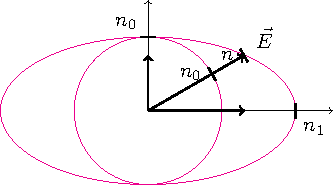
\includegraphics[width=\textwidth]{img/dvp2}
			\end{figure}
		\end{column}
	\end{columns}
\end{frame}
%%%%%%%%%%%%%%%%%%%%%%%%%%%%%%%%%%%%%%%%%%%%%%%%%%%%%%%%%%%%%
\subsection{Вращатели Фарадея}
\begin{frame}[t]
	\frametitle{Вращатель и фильтр Фарадея}
	% \framesubtitle{Вращение плоскости поляризации}
	\textbf{Вращатель Фарадея} - вещество, способное вращать плоскость поляризации в магнитном поле. \textbf{Изолятор Фарадея} - вещество, поворачивающее плоскость поляризации на $\frac{\pi}{4}$. В нашей работе вращателями Фарадея являются теллуритные стекла. 
	% \vspace{1em}
	\begin{center}
		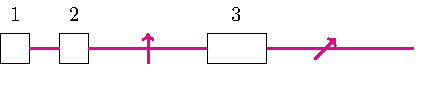
\includegraphics[width=0.8\textwidth]{img/rot}
		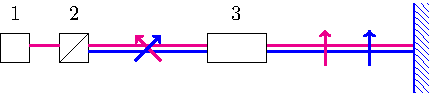
\includegraphics[width=0.8\textwidth]{img/zerc}
	\end{center}
	\begin{columns}
		\hspace{2.5cm}
		\begin{column}{0.3\textwidth}
			
			\textbf{1} -- источник
			
			\textbf{2} -- поляризатор
			
		\end{column}
		\hspace{1.6cm}
		\begin{column}{0.7\textwidth}
			
			\textbf{3} -- вращатель\\
			или фильтр Фарадея
		\end{column}
	\end{columns}
	% \textbf{1} -- источник
	
	% \textbf{2} -- поляризатор
	
	% \textbf{3} -- вращатель/фильтр Фарадея
	
\end{frame}
\begin{frame}
	\frametitle{Материальная константа: постоянная Верде}
	$V$ -- постоянная Верде -- физическая величина, характеризующая угол, на который повернется плоскость поляризации при данных длине образца и магнитном поле:
	\begin{equation}
		\Theta=V \int B(x)dx
	\end{equation}
	где $\Theta$ -- угол, на который поворачивается плоскость поляризации.
\end{frame}
%%%%%%%%%%%%%%%%%%%%%%%%%%%%%%%%%%%%%%%%%%%%%%%%%%%%%%%%%%%%%
\section{Экспериментальная часть}
\subsection{Схема установки}
\begin{frame}
	\frametitle{Схема установки}
	\begin{figure}[tb]
		\centering
		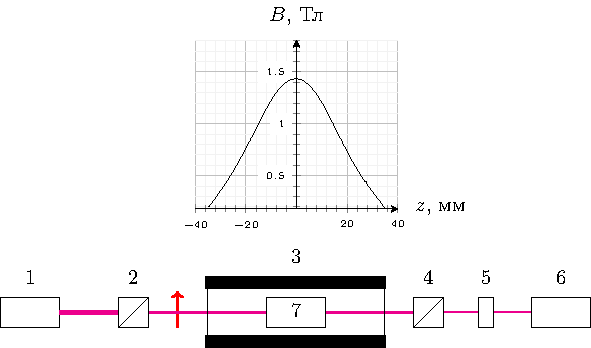
\includegraphics[width=0.8\textwidth]{img/chem}
	\end{figure}
	\begin{columns}
		\hspace{2.5cm}
		\begin{column}{0.3\textwidth}
			
			
			\textbf{1} -- диодный лазер\\ 
			$\quad\lambda_1=531$ нм,\\
			$\quad\lambda_2=658$ нм,\\
			$\quad\lambda_3=1064$ нм
			
			
			\textbf{2} -- поляризатор
			
		\end{column}
		\hspace{1.6cm}
		\begin{column}{0.7\textwidth}
			
			\textbf{3} -- магнит
			
			\textbf{4} -- призма Глана
			
			\textbf{5} -- фильтр
			
			\textbf{6} -- камера
			
			\textbf{7} -- образец
		\end{column}
	\end{columns}
	
\end{frame}
%%%%%%%%%%%%%%%%%%%%%%%%%%%%%%%%%%%%%%%%%%%%%%%%%%%%%%%%%%%%%
\subsection{Анализ результатов}
\begin{frame}[t]\frametitle{Результаты эксперимента}
	%  \begin{columns}
	%     \begin{column}{0.4\textwidth}
	
	%     \tikz{\draw[fill=magenta] (0,0) rectangle (0.5em,0.5em);} — \small{TWLTb-231/1 (l=25.8мм)}\\
	%     \tikz{\draw[fill=blue] (0,0) rectangle (0.5em,0.5em);} — \small{TWLDyB-235/4 (15,2мм)}\\
	%     \tikz{\draw[fill=black] (0,0) rectangle (0.5em,0.5em);} — \small{TWLPB-229/1 (22,5мм)}\\
	%     \tikz{\draw[fill=green] (0,0) rectangle (0.5em,0.5em);} — \small{TWLEuB-230/6 (20,2мм)}\\
	%     \tikz{\draw[fill=magenta!40!blue] (0,0) rectangle (0.5em,0.5em);} — \small{TZNDy-236/4 (24,7мм)}\\
	%     Лучший образец -- TZNDy-236/4\\
	%     Худший -- TWLTb-231/1
	% \end{column}
	% \begin{column}{0.6\textwidth}
	\begin{figure}[tb]
		\centering
		\hspace{5em}%!TEX root = presa.tex
  \begin{tikzpicture}[scale=1.1]
  \begin{axis}[
    xlabel={$\lambda$, нм},
    ylabel={$V, \frac{\text{рад}}{\text{Тл}\cdot\text{м}}$},
    domain=400:2000,
    grid=both,
    grid style={line width=.1pt, draw=gray!10},
    major grid style={line width=.2pt,draw=gray!50},
    minor y tick num=4,
    minor x tick num=4,
    xtick distance=200,
    ytick distance=5,
    ymin = 4,
    % enlargelimits={abs=0.5},
    axis line style={latex-latex},
    ticklabel style={font=\small,fill=white},    
    axis lines=middle,     
    % legend pos = north west,
    legend entries={{TWLTb-231/1},
                    {TWLDyB-235/4},
                    {TWLPB-229/1},
                    {TWLEuB-230/6},
                    {TZNDy-236/4}},
    % legend pos=outer north east    
    legend pos= north east,  
every axis x label/.style={
    at={(ticklabel* cs:1.05)},
    anchor=west,
},
every axis y label/.style={
    at={(ticklabel* cs:1.05)},
    anchor=south,
},    
   /pgf/number format/.cd,
        use comma,
        1000 sep={}]
    % legend style={
    % at={(0,0)},
    % anchor=north east,at={(axis description cs:0,-0.1)}},
    % ]

  \addlegendimage{mark=square*,color=magenta}
  \addlegendimage{mark=*,color=blue,dashed}
  \addlegendimage{mark=otimes,color=black}
  \addlegendimage{mark=triangle*,color=red}
  \addlegendimage{mark=diamond*,color=magenta!40!blue}

  \xdef\A{1.163e+04}
  \xdef\B{0.6811}
  \xdef\C{0.09754}

  \addplot[magenta]{1/x*(\A+\B/(x^2-\C^2))};    
    \addplot[color=magenta, draw=none,mark=square*] coordinates {
    (531,22.8)
    (658,13.24)
    (1064,9.36)
  };
 \xdef\A{1.35e+04} 
\xdef\B{0.5606} 
\xdef\C{0.9575} 
  \addplot[blue,dashed]{1/x*(\A+\B/(x^2-\C^2))};    
    \addplot[color=blue, draw=none,mark=*] coordinates {
    (531,31.74)
    (658,15.25)
    (1064,5.48)
  };  
\xdef\A{1.219e+04} 
\xdef\B{0.1984} 
\xdef\C{0.9706} 
  \addplot[black]{1/x*(\A+\B/(x^2-\C^2))};    
    \addplot[color=black, draw=none,mark=otimes] coordinates {
    (531,24.3)
    (658,14.05)
    (1064,10.36)
  };  
\xdef\A{1.469e+04} 
\xdef\B{0.4854} 
\xdef\C{0.8003} 
  \addplot[red]{1/x*(\A+\B/(x^2-\C^2))};    
    \addplot[color=red, draw=none,mark=triangle*] coordinates {
    (531,29.58)
    (658,17.12)
    (1064,12.79)
  };   
\xdef\A{1.679e+04} 
\xdef\B{0.4218} 
\xdef\C{0.9157}
  \addplot[magenta!40!blue]{1/x*(\A+\B/(x^2-\C^2))};    
    \addplot[color=magenta!40!blue, draw=none,mark=diamond*] coordinates {
    (531,30.77)
    (658,19.68)
    (1064,11.69)
  };        

  \end{axis}
  \end{tikzpicture}    
	\end{figure}
	%     \end{column}
	% \end{columns}
	% \centering
	% %!TEX root = presa.tex
  \begin{tikzpicture}[scale=1.1]
  \begin{axis}[
    xlabel={$\lambda$, нм},
    ylabel={$V, \frac{\text{рад}}{\text{Тл}\cdot\text{м}}$},
    domain=400:2000,
    grid=both,
    grid style={line width=.1pt, draw=gray!10},
    major grid style={line width=.2pt,draw=gray!50},
    minor y tick num=4,
    minor x tick num=4,
    xtick distance=200,
    ytick distance=5,
    ymin = 4,
    % enlargelimits={abs=0.5},
    axis line style={latex-latex},
    ticklabel style={font=\small,fill=white},    
    axis lines=middle,     
    % legend pos = north west,
    legend entries={{TWLTb-231/1},
                    {TWLDyB-235/4},
                    {TWLPB-229/1},
                    {TWLEuB-230/6},
                    {TZNDy-236/4}},
    % legend pos=outer north east    
    legend pos= north east,  
every axis x label/.style={
    at={(ticklabel* cs:1.05)},
    anchor=west,
},
every axis y label/.style={
    at={(ticklabel* cs:1.05)},
    anchor=south,
},    
   /pgf/number format/.cd,
        use comma,
        1000 sep={}]
    % legend style={
    % at={(0,0)},
    % anchor=north east,at={(axis description cs:0,-0.1)}},
    % ]

  \addlegendimage{mark=square*,color=magenta}
  \addlegendimage{mark=*,color=blue,dashed}
  \addlegendimage{mark=otimes,color=black}
  \addlegendimage{mark=triangle*,color=red}
  \addlegendimage{mark=diamond*,color=magenta!40!blue}

  \xdef\A{1.163e+04}
  \xdef\B{0.6811}
  \xdef\C{0.09754}

  \addplot[magenta]{1/x*(\A+\B/(x^2-\C^2))};    
    \addplot[color=magenta, draw=none,mark=square*] coordinates {
    (531,22.8)
    (658,13.24)
    (1064,9.36)
  };
 \xdef\A{1.35e+04} 
\xdef\B{0.5606} 
\xdef\C{0.9575} 
  \addplot[blue,dashed]{1/x*(\A+\B/(x^2-\C^2))};    
    \addplot[color=blue, draw=none,mark=*] coordinates {
    (531,31.74)
    (658,15.25)
    (1064,5.48)
  };  
\xdef\A{1.219e+04} 
\xdef\B{0.1984} 
\xdef\C{0.9706} 
  \addplot[black]{1/x*(\A+\B/(x^2-\C^2))};    
    \addplot[color=black, draw=none,mark=otimes] coordinates {
    (531,24.3)
    (658,14.05)
    (1064,10.36)
  };  
\xdef\A{1.469e+04} 
\xdef\B{0.4854} 
\xdef\C{0.8003} 
  \addplot[red]{1/x*(\A+\B/(x^2-\C^2))};    
    \addplot[color=red, draw=none,mark=triangle*] coordinates {
    (531,29.58)
    (658,17.12)
    (1064,12.79)
  };   
\xdef\A{1.679e+04} 
\xdef\B{0.4218} 
\xdef\C{0.9157}
  \addplot[magenta!40!blue]{1/x*(\A+\B/(x^2-\C^2))};    
    \addplot[color=magenta!40!blue, draw=none,mark=diamond*] coordinates {
    (531,30.77)
    (658,19.68)
    (1064,11.69)
  };        

  \end{axis}
  \end{tikzpicture}    
	% \end{frame}
	
	% \begin{frame}
	Длина образца, при к-й плоскость поляризации повернулась бы на $\frac{\pi}{4}$ -- 11см для волны 2мкм. При такой длине сказывается неоднородность поля $\Rightarrow$ образец некачественный и в данном магнитном поле не будет эффективным как изолятор Фарадея.
\end{frame}
%%%%%%%%%%%%%%%%%%%%%%%%%%%%%%%%%%%%%%%%%%%%%%%%%%%%%%%%%%%%%
\section{Выводы}
\begin{frame}
	\frametitle{Выводы}
	В ходе этого эксперимента мы 
	\begin{enumerate}
		\item исследовали магнитооптические свойства теллуритных стекол
		\item определили материальную константу -- постоянную Верде
		\item определили лучший и худший образец
		\item определили длину образца, при к-й теллуритное стекло стало бы изолятором Фарадея
	\end{enumerate}
\end{frame}

\begin{frame}[plain]
	\vspace{4cm}
	\begin{center}
		\Huge
		Спасибо за внимание!
	\end{center}
	\vspace{2.5cm}
	\begin{center}
		\color{black!30!white}
		Презентация подготовлена в издательской \\
		системе LaTeX с использованием пакетов \\
		PGF/TikZ и Beamer
	\end{center}
\end{frame}
%%%%%%%%%%%%%%%%%%%%%%%%%%%%%%%%%%%%%%%%%%%%%%%%%%%%%%%%%%%%%
\end{document}